\documentclass[12pt,a4paper]{article}
\usepackage{amsmath,amssymb,amsfonts}
\usepackage{geometry}
\geometry{margin=1in}
\usepackage{tikz}
\usetikzlibrary{angles,quotes}
\usepackage{multicol}

\title{Geometry Tools}
\author{Tutoring Centre Ferndale\\
\includegraphics[width=4em]{ApS_logo.png}}
\date{}

\begin{document}

\maketitle

\noindent

Geometry is a branch of mathematics that deals with shapes, sizes, and the properties of space. These rules and theorems of geometry are used to solve problems in geometry.\\

A clear diagram with all known values labeled allows use of these geometric rules and theorems in setting up algebraic equations that lead to a solution.

\section*{Triangles}

\subsection*{Scalene Triangle}
Scalene means uneven. Triangles with different side lengths and angles are called scalene triangles. The angles of any triangle will always add up to 180 degrees.

\begin{center}
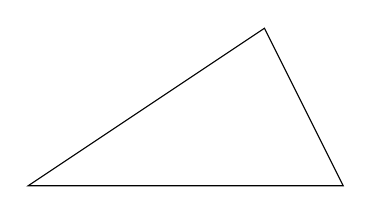
\begin{tikzpicture}
\draw (0,0) -- (4,0) -- (3,2) -- cycle;
\end{tikzpicture}
\end{center}

\subsection*{Triangle Inequality Theorem}
The sum of the lengths of any two sides of a triangle is greater than the length of the third side.

\begin{center}
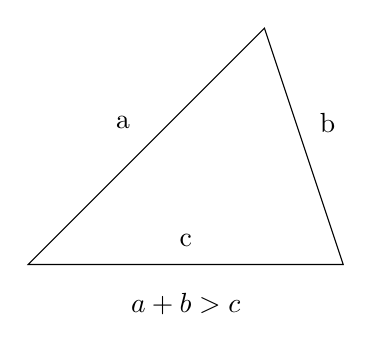
\begin{tikzpicture}
    \draw (0,0) -- (4,0) -- (3,3) -- cycle;
    \node at (2,0.3) {c};
    \node at (3.8,1.8) {b};
    \node at (1.2,1.8) {a};
    \node at (2,-0.5) {$a + b > c$};
\end{tikzpicture}
\end{center}

\newpage

\subsection*{Midpoint Theorem}
The line segment joining the midpoints of two sides of a triangle is parallel to the third side and half as long.

\begin{center}
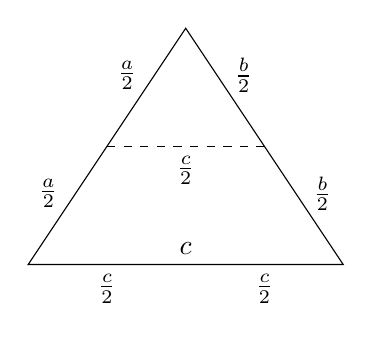
\begin{tikzpicture}
    \draw (0,0) -- (4,0) -- (2,3) -- cycle;
    \draw[dashed] (1,1.5) -- (3,1.5);
    
    \node[left] at (.5,.9) {$\frac{a}{2}$};
    \node[left] at (1.5,2.4) {$\frac{a}{2}$};
    
    \node[right] at (3.5,.9) {$\frac{b}{2}$};
    \node[right] at (2.5,2.4) {$\frac{b}{2}$};
    
    \node[below] at (1,0) {$\frac{c}{2}$};
    \node[below] at (3,0) {$\frac{c}{2}$};

    \node[below] at (2,1.5) {$\frac{c}{2}$};
    \node[above] at (2,0) {$c$};
\end{tikzpicture}
\end{center}

\subsection*{Exterior Angle Theorem}
The measure of an exterior angle of a triangle is equal to the sum of the measures of the two non-adjacent interior angles.

\begin{center}
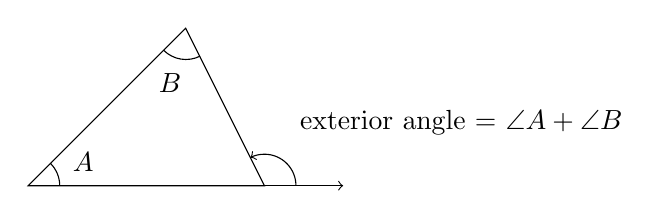
\begin{tikzpicture}
    \draw (0,0) -- (3,0) -- (2,2) -- cycle;
    \draw[thin] (0.4,0) arc[start angle=0, end angle=45, radius=0.4];
    \node at (0.7,0.3) {$A$};
    \draw[thin] (1.72,1.72) arc[start angle=225, end angle=296.56, radius=0.4];
    \node at (1.8,1.3) {$B$};
    \draw[->] (3,0) -- (4,0);
    \draw[->,thin](3.4,0) arc[start angle=0, end angle=116.56, radius=0.4];
    \node at (5.5,0.8) {exterior angle = $\angle A + \angle B$};
\end{tikzpicture}
\end{center}

\subsection*{Angle Bisector Theorem}
In a triangle, the bisector of an angle divides the opposite side into two segments that are proportional to the lengths of the other two sides.


\begin{center}
\begin{tikzpicture}
\draw (0,0) --(5,5) node[midway, above]{$a$};
\draw (5,5) --(4,1) node[midway, right]{$b$};
\draw[dashed] (5,5) -- (2,0.5);
\draw[thin] (4.29,4.29) arc[start angle = 225, end angle = 255.96, radius=1];
\node at (3.7,3.4) {$\theta$};
\node at (4.2,3.2) {$\theta$};
\draw (4,1) --(2,0.5) node[midway, below]{$y$};
\draw (2,0.5) --(0,0) node[midway, below]{$x$};
\node at (7,3) {\Large{$\frac{a}{b} = \frac{x}{y}$}};
\end{tikzpicture}
\end{center}

\newpage

\subsection*{Centroid Theorem}

\begin{itemize}
    \item A median of a triangle is a line segment drawn from a vertex to the midpoint of the opposite side.
    \item The centroid of a triangle is the point where all three medians intersect.    
\end{itemize}

\begin{center}
\begin{minipage}{0.48\textwidth}
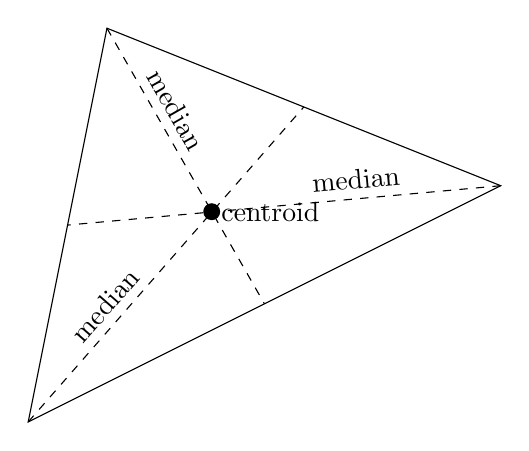
\begin{tikzpicture}
\draw (0,0) -- (1,5) -- (6,3) -- cycle;
\draw [dashed] (0,0) -- (3.5,4) node [pos=0.33,sloped,above] {median};
\draw [dashed] (1,5) -- (3,1.5) node [pos=0.33,sloped,above] {median};
\draw [dashed] (6,3) -- (0.5,2.5) node [pos=0.33,sloped,above] {median};
\draw [fill] (2.33,2.67) circle (0.1) node [right] {centroid};
\end{tikzpicture}
\end{minipage}
\hfill
\begin{minipage}{0.48\textwidth}
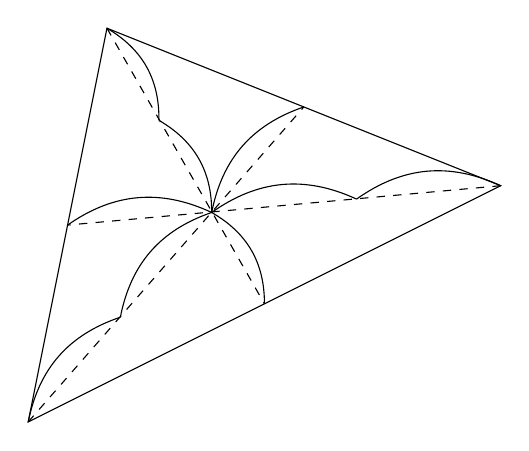
\begin{tikzpicture}
\draw (0,0) -- (1,5) -- (6,3) -- cycle;
\draw [dashed] (0,0) -- (3.5,4);
\draw [dashed] (1,5) -- (3,1.5);
\draw [dashed] (6,3) -- (0.5,2.5);
\draw [thin] (1,5) to [bend left=30] (1.66,3.83);
\draw [thin] (1.66,3.83) to [bend left=30] (2.33,2.66);
\draw [thin] (2.33,2.66) to [bend left=30] (3,1.5);
\draw [thin] (0.5,2.5) to [bend left=30] (2.33,2.66);
\draw [thin] (2.33,2.66) to [bend left=30] (4.17,2.83);
\draw [thin] (4.17,2.83) to [bend left=30] (6,3);
\draw [thin] (0,0) to [bend left=30] (1.17,1.33);
\draw [thin] (1.17,1.33) to [bend left=30] (2.33,2.66);
\draw [thin] (2.33,2.66) to [bend left=30] (3.5,4);
\end{tikzpicture}
\end{minipage}
\end{center}

The centroid of a triangle divides each median into two segments in the ratio \(2:1\), with the longer segment being closer to the vertex.

\subsection*{Similar Triangles}
Two triangles are said to be similar if they have the same shape but not necessarily the same size. This means that:

\begin{itemize}
    \item \textbf{Corresponding angles are equal.}
    \item \textbf{Corresponding sides are proportional.}
\end{itemize}

If \(\triangle ABC\) and \(\triangle DEF\) are similar, we write:
\[
\triangle ABC \sim \triangle DEF
\]

Two triangles are similar if any one of the following criteria is true:
\begin{enumerate}
    \item \textbf{AA (Angle-Angle):} If two angles of one triangle are equal to two angles of another triangle.
    \item \textbf{SSS (Side-Side-Side):} If the corresponding sides of two triangles are proportional.
    \item \textbf{SAS (Side-Angle-Side):} If one angle of a triangle is equal to one angle of another triangle, and the sides including these angles are proportional.
\end{enumerate}

\newpage

\subsection*{Congruent Triangles}
Two triangles are said to be congruent if they have the same shape and the same size. This means that:

\begin{itemize}
    \item \textbf{All corresponding angles are equal.}
    \item \textbf{All corresponding sides are equal.}
\end{itemize}

If \(\triangle ABC\) and \(\triangle DEF\) are congruent, we write:
\[
\triangle ABC \cong \triangle DEF
\]

Two triangles are congruent if any one of the following criteria is true:
\begin{enumerate}
    \item \textbf{SSS (Side-Side-Side):} All three sides of one triangle are equal to all three sides of another triangle.
    \item \textbf{SAS (Side-Angle-Side):} Two sides and the angle between them in one triangle are equal to two sides and the angle between them in another triangle.
    \item \textbf{ASA (Angle-Side-Angle):} Two angles and the side between them in one triangle are equal to two angles and the side between them in another triangle.
    \item \textbf{AAS (Angle-Angle-Side):} Two angles and a non-included side in one triangle are equal to two angles and a corresponding non-included side in another triangle.
    \item \textbf{RHS (Right angle-Hypotenuse-Side):} In right-angled triangles, the hypotenuse and one side of one triangle are equal to the hypotenuse and one side of another triangle.
\end{enumerate}

\newpage

\section*{Trigonometry}

The sides of a right triangle are named relative to the angle $\theta$ in standard position on the unit circle:

\begin{center}
\begin{minipage}{0.45\textwidth}
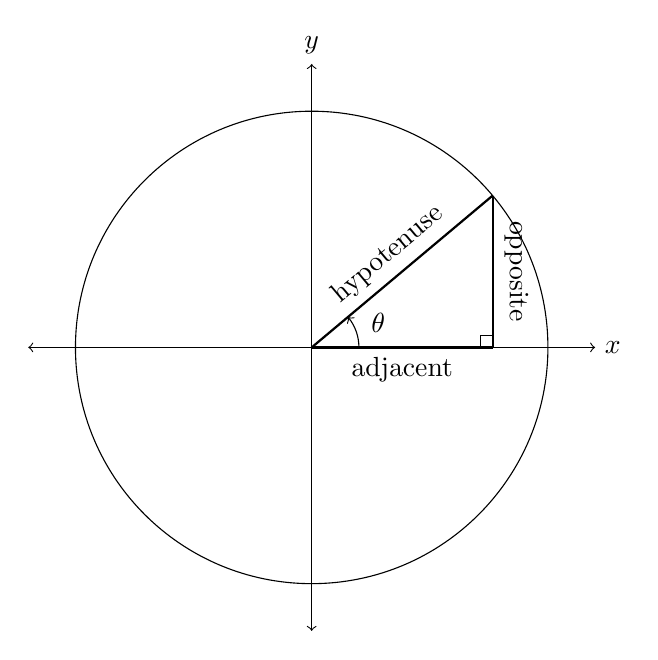
\begin{tikzpicture}[scale=3]
    \draw[<->] (-1.2,0) -- (1.2,0) node[right] {$x$};
    \draw[<->] (0,-1.2) -- (0,1.2) node[above] {$y$};
    \draw[thin] (0,0) circle(1);
    \draw[thick] (0,0) -- ({cos(40)}, {sin(40)}) node[midway, sloped, above]{hypotenuse};
    \draw[thick] ({cos(40)}, {sin(40)}) -- ({cos(40)}, 0) node[midway,xshift=2ex,rotate=270]{opposite};
    \draw[thick] ({cos(40)}, 0) -- (0,0) node[midway, sloped, below]{adjacent};
    \draw[thin,->] (0.2,0) arc (0:40:0.2);
    \node at (20:0.3) {$\theta$};
    \draw[thin] ({cos(40)-0.05}, 0) -- ({cos(40)-0.05}, 0.05) -- ({cos(40)}, 0.05);
\end{tikzpicture}
\end{minipage}
\begin{minipage}{0.45\textwidth}
\begin{tikzpicture}[scale=3]
    \draw[thin] (0,0) circle(1);
    \draw[->, thick] (0,0) -- (1,0)
    node[anchor=north west] {1};
    \draw[->, thick] (0,0) -- ({cos(30)}, {sin(30)}) node[anchor=south west] {$(\cos \theta, \sin \theta)$};
    \draw[->,thin] (0.2,0) arc (0:30:0.2);
    \node at (15:0.3) {$\theta$};
    \draw[dashed](0,{sin(30)}) -- ({cos(30)},{sin(30})
    node[midway,sloped,above]{cosine};
    \draw[dashed]({cos(30)},0) -- ({cos(30)},{sin(30)})
    node[midway,sloped,above]{sine};
    \draw[<->] (-1.2,0) -- (1.2,0) node[right] {$x$};
    \draw[<->] (0,-1.2) -- (0,1.2) node[above] {$y$};
\end{tikzpicture}
\end{minipage}
\end{center}

\textbf{SOHCAHTOA} stands for:
\begin{center}
\textbf{SOH:} Sine $= \frac{\textrm{Opposite}}{\textrm{Hypotenuse}}$\\
\vspace{8pt}
\textbf{CAH:} Cosine $= \frac{\textrm{Adjacent}}{\textrm{Hypotenuse}}$\\
\vspace{8pt}
\textbf{TOA:} Tangent $= \frac{\textrm{Opposite}}{\textrm{Adjacent}}$\\
\end{center}

\subsection*{Sine Rule}
\[ \frac{a}{\sin A} = \frac{b}{\sin B} = \frac{c}{\sin C} \]

\subsection*{Cosine Rule}
\[ c^2 = a^2 + b^2 - 2ab \cos C \]

\begin{center}
\begin{tikzpicture}[scale=1.5]
    \draw(0,0)--(5,3)node[midway,above]{$a$};
    \draw(0,0)--(4,1)node[midway,below]{$b$};
    \draw(4,1)--(5,3)node[midway,right]{$c$};
    \draw[thin] (4.13, 1.27) arc[start angle=63.43, end angle=194.04, radius=0.3]; % Arc for angle A at (4,1)
    \draw[thin] (4.57, 2.74) arc[start angle=210.96, end angle=243.43, radius=0.5]; % Arc for angle B at (5,3)
    \draw[thin] (0.78, 0.19) arc[start angle=14.04, end angle=30.96, radius=0.8]; % Arc for angle C at (0,0)
    \node at (3.6,1.3){$A$};
    \node at (4.3,2.3){$B$};
    \node at (1.5,0.6){$C$};
\end{tikzpicture}
\end{center}
where \( a \), \( b \), and \( c \) are the lengths of the sides of the triangle, and \( A \), \( B \), and \( C \) are the opposite angles.

\subsection*{Triangle Configurations: SSS, SAS, AAS, ASA, RHS}

\subsubsection*{SSS (Side-Side-Side)}
In the SSS configuration, all three sides of the triangle are known. This allows us to use the \textit{Cosine Rule} to determine the angles of the triangle.

\subsubsection*{SAS (Side-Angle-Side)}
In the SAS configuration, two sides and the included angle (the angle between the two sides) are known. This allows us to use the \textit{Cosine Rule} to find the third side or the other angles.

\subsubsection*{AAS (Angle-Angle-Side)}
In the AAS configuration, two angles and one side (with the side not between the angles) are known. This allows us to use the \textit{Sine Rule} to find the remaining sides or angles.

\subsubsection*{ASA (Angle-Side-Angle)}
In the ASA configuration, two angles and the included side (the side between the two angles) are known. This can be solved using the \textit{Sine Rule} or the \textit{Cosine Rule} (if needed).

\subsubsection*{RHS (Right Angle-Hypotenuse-Side)}
In the RHS configuration, a right-angled triangle is known, with the hypotenuse and one side given. This allows us to use basic trigonometric ratios (sine, cosine, and tangent) to find the other sides or angles.

\section*{Special Triangles}\label{sec:special-triangles}
\subsection*{Equilateral Triangle}
Equilateral means equal sides. An equilateral triangle has three equal sides and three equal angles. Each angle measures $60^\circ$.

\begin{center}
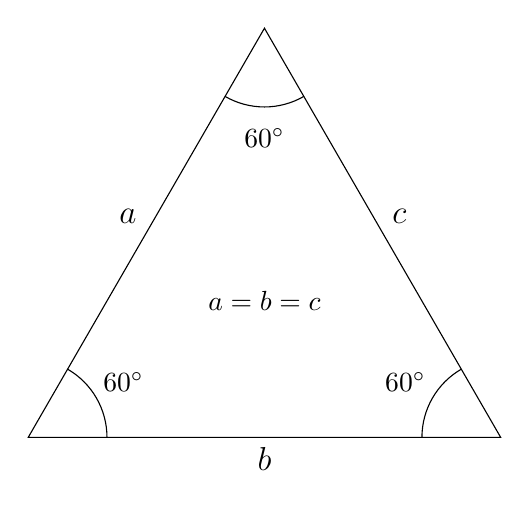
\begin{tikzpicture}
    \draw (0,0) -- (6,0) node[midway,below] {\large{$b$}} -- (3,5.196)  node[midway,above right] {\large{$c$}} -- cycle  node[midway,above left] {\large{$a$}};
    \node at (3,1.732) {$a=b=c$};
    \draw (1,0) arc [start angle=0,end angle=60,radius=1];
    \draw (5.5,0.866) arc [start angle=120,end angle=180,radius=1];
    \draw (2.5,4.33) arc [start angle=240,end angle=300,radius=1];
    \node at (1.21,.7) {$60^\circ$};
    \node at (3,3.8) {$60^\circ$};
    \node at (4.79,.7) {$60^\circ$};
\end{tikzpicture}
\end{center}

\subsection*{Isosceles Triangle}
Isosceles means equal legs. An isosceles triangle has two equal sides, and the angles opposite these sides are also equal. An isosceles triangle can be bisected to make two right triangles.

\begin{center}
    \begin{tikzpicture}
        \draw (0,0) -- (6,0)
        node [midway, below] {\large{$b$}}
        -- (3,4) node [midway, above right] {\large{$c$}}
        -- cycle node [midway, above left] {\large{$a$}};
        \node at (4.96,0.6){$A$};
        \node at (3.2,2.8){$B$};
        \node at (1.04,0.6){$C$};
        \draw (1,0) arc[start angle=0,end angle=53.13,radius=1];
        \draw (5,0) arc[start angle=180,end angle=126.87,radius=1];
        \draw (2.4,3.2) arc[start angle=233.13,end angle=306.87,radius=1];
        \draw[dashed] (3,0) -- (3,4);
        \draw[fine] (3.3,0) -- (3.3,0.3) -- (3,0.3);
        \node[right] at (6,3) {\large{$a=c$}};
        \node[right] at (6,2.5) {\large{$\angle C=\angle A$}};
    \end{tikzpicture}
\end{center}

\subsection*{Right Triangle}
A right triangle has one angle equal to $90^\circ$. The side of a right triangle opposite the right angle is called the hypotenuse, which is the longest side. Hypotenuse means stretched under (the right angle.) The other two sides of a right triangle are called legs.

\begin{center}
\begin{tikzpicture}
    \draw (0,0) -- (3,0) node[sloped,midway,below] {leg};
    \draw (3,0) -- (0,4) node [sloped,midway,above] {hypotenuse};
    \draw (0,4) -- (0,0) node[midway,left] {leg};
    \draw[fine] (0.3,0) -- (0.3,0.3) -- (0,0.3);
    \node[above right] at (0.3,0.3) {$90^\circ$};
\end{tikzpicture}
\end{center}

\subsubsection*{Similar Right Triangles}
Given a right triangle \( \triangle ABC \) where \( \angle C = 90^\circ \) and a perpendicular line drawn from \( C \) to a point \( C_1 \) on the hypotenuse \( AB \), two smaller similar right triangles, \( \triangle ACC_1 \) and \( \triangle BCC_1 \) are created. They are similar (same angles and side lengths in proportion) to each other and to the original right triangle.

\begin{center}
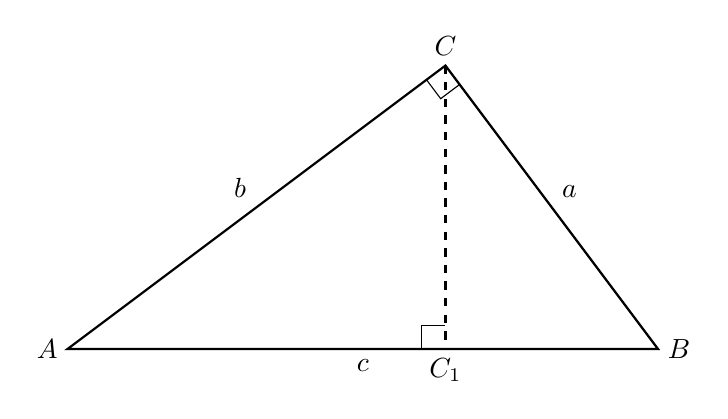
\begin{tikzpicture}[scale=1.5]
\coordinate [label=left:$A$] (A) at (0,0);
\coordinate [label=above:$C$] (C) at (3.2,2.4);
\coordinate [label=right:$B$] (B) at (5,0);
\coordinate [label=below:$C_1$] (C1) at (3.2,0);
\draw [thick] (A) -- node[midway, below]{$c$} (B) -- node[midway, above right]{$a$} (C) -- node[midway, above left]{$b$} cycle;
\draw [thick, dashed] (C) -- (C1);
\draw [thin] (3,0) -- (3,.2) -- (3.2,.2);
\draw [thin] (3.04,2.28) -- (3.16,2.12) -- (3.32,2.24);
\end{tikzpicture}
\end{center}

\subsection*{The Pythagorean Theorem}
The Pythagorean Theorem applies to right triangles:
\[ a^2 + b^2 = c^2, \]
where $a$ and $b$ are the lengths of the legs, and $c$ is the length of the hypotenuse.\\

If you draw squares on each of the three sides of the triangle, the sum of the areas of the two smaller rectangles equals the area of the square on the hypotenuse.

\begin{figure}[h!]
    \centering
    \begin{tikzpicture}
        \draw[thick] (0, 0) -- (3, 0) node[midway, below] {$a$};
        \draw[thick] (3, 0) -- (3, 4) node[midway, right] {$b$};
        \draw[thick] (3, 4) -- (0, 0) node[midway, left] {$c$} node[midway, sloped, below] {\tiny{hypotenuse}};
        \draw (2.7, 0) -- (2.7, 0.3) -- (3, 0.3);
        \node[above left] at (2.8, 0.2) {\tiny{$90^\circ$}};
        \draw[thick] (0, 0) -- (0,-3) -- (3,-3) -- (3, 0); \node at (1.5,-1.5) {$a^2$};
        \draw[thick] (3, 0) -- (7, 0) -- (7, 4) -- (3, 4); \node at (5, 2)     {$b^2$};
        \draw[thick] (0, 0) -- (-4,3) -- (-1,7) -- (3, 4); \node at (-0.5,3.5) {$c^2$};
    \end{tikzpicture}
\end{figure}

\subsection*{30-60-90 Triangle}

A $30$-$60$-$90$ triangle is a special type of right triangle where the angles are $30^\circ$, $60^\circ$, and $90^\circ$. The sides are in the ratio:
\[ 1 : \sqrt{3} : 2, \]
where the shortest side is opposite the $30^\circ$ angle, the longer leg is opposite the $60^\circ$ angle, and the hypotenuse is twice the length of the shortest side.

\begin{center}
    \begin{tikzpicture}
        \draw (0,0) -- (5.196,0) node[midway, below] {\large{$2$}};
        \draw (5.196,0) -- (0,3) node[midway, above right] {\large{$\sqrt{3}$}};
        \draw (0,3) -- (0,0) node[midway, left] {\large{$1$}};
        \draw[thin] (0.3,0) -- (0.3,0.3) -- (0,0.3);
        \node at (0.7,0.5) {\large{$90^\circ$}}
        \draw (4.5,0) arc [start angle=180,end angle=150,radius=0.7];
        \node at (3.8,0.4) {\large{$30^\circ$}}
        \draw (0,2.5) arc [start angle=270,end angle=330,radius=0.5];
        \node at (0.6,2.2) {\large{$60^\circ$}}
    \end{tikzpicture}
\end{center}

These properties allow you to quickly find the lengths of all sides of a 30-60-90 triangle if you know the length of just one side.

\subsection*{45-45-90 Triangle}
A $45$-$45$-$90$ triangle is a special type of right triangle where the angles are $45^\circ$, $45^\circ$, and $90^\circ$. The sides are in the ratio:
\[ 1 : 1 : \sqrt{2}, \]
where the legs are of equal length, and the hypotenuse is $\sqrt{2}$ times the length of a leg.

\begin{center}
    \begin{tikzpicture}
        \draw (0,0) -- (4,0) node[midway, below] {{\large$1$}};
        \draw (4,0) -- (0,4) node[midway, above right] {\large${\sqrt{2}}$};
        \draw (0,4) -- (0,0) node[midway, left] {\large{$1$}};
        \draw[thin] (0.3,0) -- (0.3,0.3) -- (0,0.3);
        \node at (0.7,0.7) {\large{$90^\circ$}}
        \draw [thin] (0,3.5) arc [start angle=270,end angle=315,radius=0.5];
        \node at (0.4,3) {\large{$45^\circ$}}
        \draw [thin] (3.5,0) arc [start angle=180,end angle=135,radius=0.5];
        \node at (3,0.4) {\large{$60^\circ$}}
    \end{tikzpicture}
\end{center}

\subsection*{Pythagorean Triples}
A \textbf{3-4-5 triangle} is a right triangle with side lengths in the ratio \(3 : 4 : 5\).
\[ 3^2 + 4^2 = 9 + 16 = 25 = 5^2. \]

Other useful integer side length combinations that form right triangles include:
\begin{itemize}
    \item \textbf{5-12-13 Triangle:}
    \[ 5^2 + 12^2 = 25 + 144 = 169 = 13^2. \]
    \item \textbf{7-24-25 Triangle:}
    \[ 7^2 + 24^2 = 49 + 576 = 625 = 25^2. \]
    \item \textbf{8-15-17 Triangle:}
    \[ 8^2 + 15^2 = 64 + 225 = 289 = 17^2. \]
\end{itemize}

These integer side lengths are known as \textbf{Pythagorean triples}. They are especially helpful in constructing or verifying right triangles.

\section*{Angles}

\subsection*{Angles Around a Point}
The sum of angles around a point is $360^\circ$.

\subsection*{Angles in a Polygon}
The sum of the interior angles of an $n$-sided polygon is given by:
\[
(n-2) \times 180^\circ.
\]
Each interior angle of a regular polygon (where all sides and angles are equal) can be calculated as:
\[
\text{Interior angle} = \frac{(n-2) \times 180^\circ}{n}.
\]

\subsection*{Complementary and Supplementary Angles}
\begin{itemize}
    \item \textbf{Complementary Angles:} Two angles are complementary if their sum is $90^\circ$.

\begin{center}
    \begin{tikzpicture}
        \draw (0,3)--(0,0)--(3,0);
        \draw (0,0)--(1.33,3);
        \draw (0.3,0) arc [0:78.69:0.3];
        \draw (0.078,0.39) arc [78.69:90:0.4];
        \node at (0.3,1.4){$\theta{_1}$}
        \node at (1,0.5){$\theta{_2}$}
        \node at (3,1) {$\theta{_1}+\theta{_2}=90^{\circ}$}
    \end{tikzpicture}
\end{center}

    \item \textbf{Supplementary Angles:} Two angles are supplementary if their sum is $180^\circ$.

\begin{center}
    \begin{tikzpicture}
        \draw (0,0)--(5,0);
        \draw (2,0)--(3,3);
        \draw (2.3,0) arc [0:78.69:0.3];
        \draw (1.6,0) arc [78.69:180:0.4];
        \node at (2.5,0.3){$\theta{_1}$}
        \node at (1.7,0.3){$\theta{_2}$}
        \node at (4,1) {$\theta{_1}+\theta{_2}=180^{\circ}$}
    \end{tikzpicture}
\end{center}

\end{itemize}

\subsection*{Vertically Opposite Angles}
When two straight lines intersect, the angles opposite each other at the point of intersection are equal.
\begin{center}
    \begin{tikzpicture}
        \draw (0,0) -- (5,4);
        \draw (0,4) -- (5,0);
        \draw [->](4.1,3.2) arc[start angle=36.87,end angle=143.13,radius=2] node[midway,above]{\large{$a$}};
        \draw [->](1.7,2.6) arc[start angle=143.13,end angle=216.87,radius=1] node[midway,left]{\large{$c$}};
        \draw [->](0.9,0.8) arc[start angle=216.87,end angle=323.13,radius=2] node[midway,below]{\large{$b$}};
        \draw [->](3.3,1.4) arc[start angle=323.13,end angle=396.87,radius=1] node[midway,right]{\large{$d$}};
        \node at (6,3) {\large{$\angle a = \angle b$}}
        \node at (6,2.4) {\large{$\angle c = \angle d$}}
    \end{tikzpicture}
\end{center}

\subsection*{Parallel Lines and Transversals}

\begin{itemize}
    \item \textbf{Corresponding angles are equal.}

\begin{center}
    \begin{tikzpicture}[scale=1.2]
        \draw (0,0) -- (4,0);
        \draw (0,1) -- (4,1);
        \draw (1,-0.5) -- (3,1.5);
        \draw (2.8,1) arc (0:45:0.3);
        \node at (3,1.2) {$\theta$};
        \draw (1.2,0) arc (180:225:0.3);
        \node at (1,-0.2) {$\theta$};
    \end{tikzpicture}
\end{center}

\newpage

\item \textbf{Alternate interior angles are equal.}

\begin{center}    
    \begin{tikzpicture}[scale=1.2]
        \draw (0,0) -- (4,0);
        \draw (0,1) -- (4,1);
        \draw (1,-0.5) -- (3,1.5);
        \draw (2.8,1) arc (0:45:0.3);
        \node at (3,1.2) {$\theta$};
        \draw (1.8,0) arc (0:45:0.3);
        \node at (2,0.2) {$\theta$};
    \end{tikzpicture}
\end{center}

    \item \textbf{Consecutive interior angles are supplementary.}
    
\begin{center}
    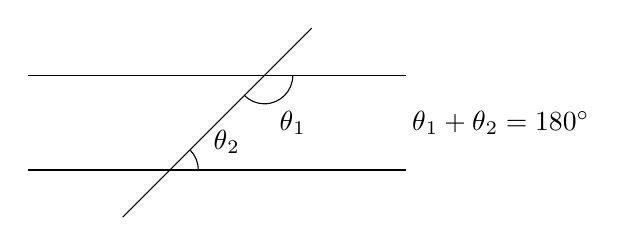
\begin{tikzpicture}[scale=1.2]
        \draw (0,0) -- (4,0);
        \draw (0,1) -- (4,1);
        \draw (1,-0.5) -- (3,1.5);

        \draw (2.8,1) arc (0:-135:0.3);
        \node at (2.8,0.5) {$\theta{_1}$};

        \draw (1.8,0) arc (0:45:0.3);
        \node at (2.1,0.3) {$\theta{_2}$};
        \node at (5,0.5) {$\theta{_1} + \theta{_2} = 180^\circ$};
    \end{tikzpicture}
\end{center}
\end{itemize}

\section*{Circles}

\subsection*{Inscribed Angle Theorem}

\begin{itemize}
\item A central angle in a circle is an angle whose vertex is at the center of the circle and whose sides (rays) extend to the circumference.
\item An inscribed angle in a circle is an angle whose vertex is on the circumference of the circle and whose sides (chords) intersect the circle.
\end{itemize}
\[ \theta = 2 \alpha \]
The measure of a central angle $\theta$ is twice the measure of an inscribed angle $\alpha$ subtending the same arc.

\begin{center}
    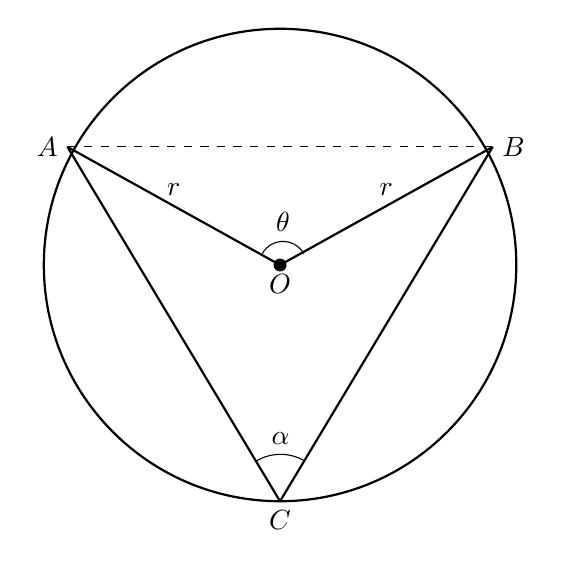
\begin{tikzpicture}[scale=1.5]
        \draw[thick] (0,0) circle(2);
        \draw[fill] (0,0) circle(0.05);
        \coordinate (O) at (0,0);
        \coordinate (A) at (-1.8,1);
        \coordinate (B) at (1.8,1);
        \coordinate (C) at (0,-2);
        \draw[thick] (O) -- (A) node[midway, above] {$r$};
        \draw[thick] (O) -- (B) node[midway, above] {$r$};
        \draw[thick] (A) -- (C);
        \draw[thick] (B) -- (C);
        \draw[dashed] (A) -- (B);
        \draw (0.2,0.097) arc[start angle=29.055, end angle=150.945, radius=0.2] node[midway, above] {$\theta$};
        \draw (0.21,-1.66) arc[start angle=59.04, end angle=120.96, radius=0.4] node[midway, above] {$\alpha$};
        \node[left] at (A) {$A$};
        \node[right] at (B) {$B$};
        \node[below] at (C) {$C$};
        \node[below] at (O) {$O$};
    \end{tikzpicture}
\end{center}

\newpage

\subsection*{Angles in the Same Segment Theorem}
Angles subtended by the same chord on the same segment of a circle are equal. This follows from the inscribed angle theorem.

\begin{center}
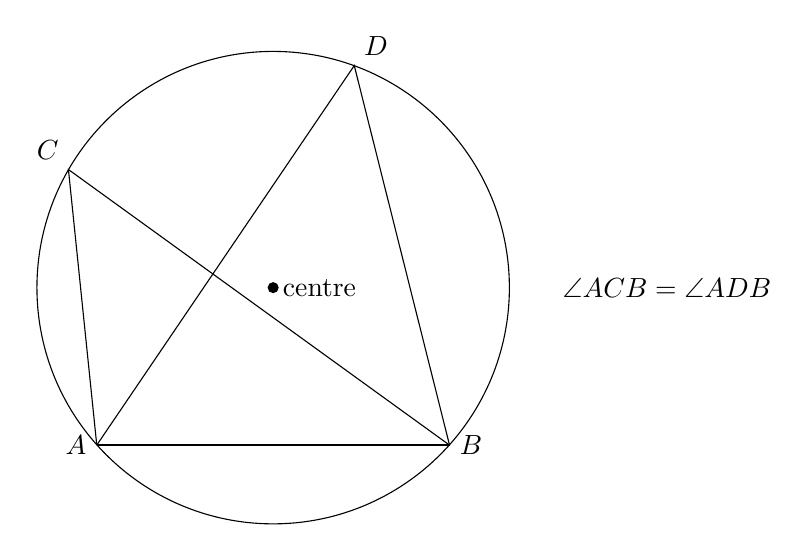
\begin{tikzpicture}
    \draw (0,0) circle [radius=3];
    \fill (0,0) circle (2pt) node[right] {centre};
    \draw [thick] (-2.24,-2) node[left] {$A$} -- (2.24,-2) node[right] {$B$};
    
    \draw (-2.24,-2) -- (-2.6,1.5) node[above left] {$C$} -- (2.24,-2);
    \draw (-2.24,-2) -- (1.03,2.82) node[above right] {$D$} -- (2.24,-2);
    \node at (5,0) {$\angle ACB = \angle ADB$};
\end{tikzpicture}
\end{center}

\subsection*{Thale's Theorem}
Thales' Theorem states that the angle subtended by a diameter at the circumference is $90^\circ$. This is a special case of the inscribed angle theorem.

\begin{center}
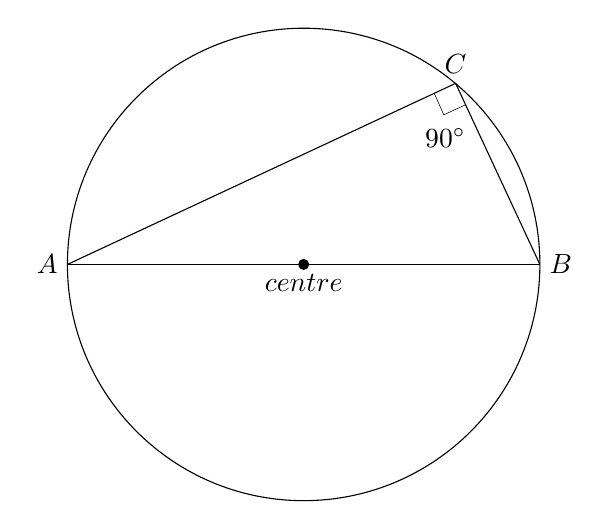
\begin{tikzpicture}
    \draw (0,0) circle [radius=3];
    \fill (0,0) circle (2pt) node[below] {$centre$};
    \draw (-3,0) -- (3,0);
    \draw (-3,0) node[left]{$A$} -- (3,0) node[right]{$B$};
    \draw (-3,0) -- (1.93,2.3) node[above]{$C$} -- (3,0);
    \draw [very thin] (1.66,2.17) -- (1.78,1.9) -- (2.06,2.03);
    \node at (1.8,1.6) {$90^\circ$};
\end{tikzpicture}
\end{center}

\newpage

\subsection*{Chord Perpendicular Bisector Theorem}
The perpendicular from the centre of a circle to a chord bisects the chord.

\begin{center}
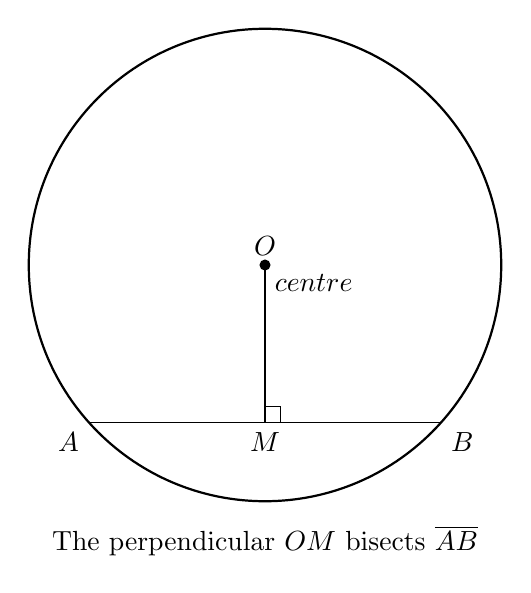
\begin{tikzpicture}
    \draw[thick] (0,0) circle [radius=3cm];
    \fill (0,0) circle (2pt) node[below right] {$centre$};
    \coordinate [label=above:$O$] (O) at (0,0);
    \coordinate [label=below left:$A$] (A) at (-2.24,-2);
    \coordinate [label=below right:$B$] (B) at (2.24,-2);
    \coordinate [label=below:$M$] (M) at (0,-2);
    \draw (A) -- (B);
    \draw (O) -- (M);
    \draw [very thin] (0,-2) ++(0.2,0) -- ++(0,0.2) -- ++(-0.2,0);
    \node at (0,-3.5) {The perpendicular $OM$ bisects $\overline{AB}$};
\end{tikzpicture}
\end{center}

\subsection*{Equal Tangents Theorem}
Tangents drawn from an external point to a circle are equal in length, and a line drawn from their intersection to the centre of the circle bisects the angle between the two tangents.

\begin{center}
\begin{tikzpicture}
    \draw (0,0) circle [radius=3cm];
    \fill (0,0) circle (2pt) node[left] {$O$};
    \draw (0,0) -- (1.92,2.3) node[above] {$A$};;
    \draw (0,0) -- (1.92,-2.3) node[below] {$B$};;
    \draw (1.92,2.3) --  (4.67,0) node[right] {$C$};
    \draw (1.92,-2.3) --(4.67,0);
    \draw[very thin,rotate around={230:(1.92,2.3)}] (1.92,2.3) rectangle ++(0.3,0.3);
    \draw[very thin,rotate around={40:(1.92,-2.3)}] (1.92,-2.3) rectangle ++(0.3,0.3);
    \node at (5,2) {$\overline{AC}=\overline{BC}$};
\end{tikzpicture}
\end{center}

\newpage

\section*{Apollonius' Theorem}
Apollonius' Theorem is a generalization of the Pythagorean Theorem for triangles that are not necessarily right-angled.

The sum of squares of any two sides of a triangle equals twice its square on half of the third side, plus twice its square on the median bisecting the third side:

\[ a^2+b^2=2(m^2+e^2) \]

\begin{center}
    \begin{tikzpicture}
        \draw (0,0) -- (4,0) node[midway,above]{\large{$e$}};
        \draw (4,0) -- (8,0) node[midway,above]{\large{$e$}};
        \draw (8,0) -- (3,3) node[midway,above right]{\large{$b$}};
        \draw (3,3) -- (0,0) node[midway,above left]{\large{$a$}};
        \draw (3,3) -- (4,0) node[midway,right]{\large{$m$}};
`        \node[below] at (4,0) {\large{$c$}};
    \end{tikzpicture}
\end{center}

\section*{Stewart's Theorem}
\begin{itemize}
    \item A cevian is a line from a corner of a triangle to the opposite side.
\end{itemize}
If a cevian divides a side of of a triangle into two segments of length m and n, with m adjacent to c and n adjacent to b, then:
\[b^{2}m+c^{2}n=a(d^{2}+mn)\]

(These terms can be rearranged to form the mnemonic $man + dad = bmb +cnc$ ("A man and his dad put a bomb in the sink.")

\begin{center}
    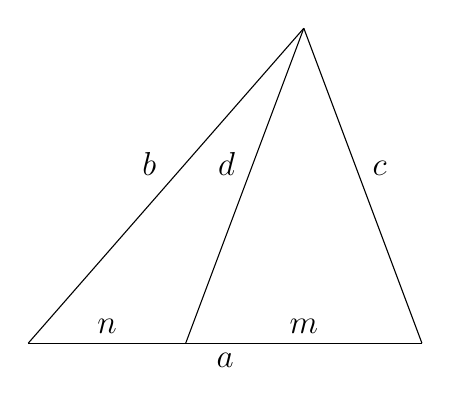
\begin{tikzpicture}
        \draw (0,0) -- (2,0) node[midway,above]{\large{$n$}};
        \draw (2,0) -- (5,0) node[midway,above]{\large{$m$}};
        \draw (5,0) -- (3.5,4) node[midway,above right]{\large{$c$}};
        \draw (3.5,4) -- (0,0) node[midway,above left]{\large{$b$}};
        \draw (3.5,4) -- (2,0) node[midway,above left]{\large{$d$}};
        \node[below] at (2.5,0) {\large{$a$}};
    \end{tikzpicture}
\end{center}

Stewart's Theorem is a generalization of Apollonius' Theorem, which is itself a generalization of Pythagoras' Theorem.

\end{document}
